% Template for Cogsci submission with R Markdown

% Stuff changed from original Markdown PLOS Template
\documentclass[10pt, letterpaper]{article}

\usepackage{cogsci}
\usepackage{pslatex}
\usepackage{float}
\usepackage{caption}

% amsmath package, useful for mathematical formulas
\usepackage{amsmath}

% amssymb package, useful for mathematical symbols
\usepackage{amssymb}

% hyperref package, useful for hyperlinks
\usepackage{hyperref}

% graphicx package, useful for including eps and pdf graphics
% include graphics with the command \includegraphics
\usepackage{graphicx}

% Sweave(-like)
\usepackage{fancyvrb}
\DefineVerbatimEnvironment{Sinput}{Verbatim}{fontshape=sl}
\DefineVerbatimEnvironment{Soutput}{Verbatim}{}
\DefineVerbatimEnvironment{Scode}{Verbatim}{fontshape=sl}
\newenvironment{Schunk}{}{}
\DefineVerbatimEnvironment{Code}{Verbatim}{}
\DefineVerbatimEnvironment{CodeInput}{Verbatim}{fontshape=sl}
\DefineVerbatimEnvironment{CodeOutput}{Verbatim}{}
\newenvironment{CodeChunk}{}{}

% cite package, to clean up citations in the main text. Do not remove.
\usepackage{apacite}

% KM added 1/4/18 to allow control of blind submission


\usepackage{color}

% Use doublespacing - comment out for single spacing
%\usepackage{setspace}
%\doublespacing


% % Text layout
% \topmargin 0.0cm
% \oddsidemargin 0.5cm
% \evensidemargin 0.5cm
% \textwidth 16cm
% \textheight 21cm

\title{How to Make a Proceedings Paper Submission}


\author{{\large \bf Morton Ann Gernsbacher (MAG@Macc.Wisc.Edu)} \\ Department of Psychology, 1202 W. Johnson Street \\ Madison, WI 53706 USA \AND {\large \bf Sharon J.~Derry (SDJ@Macc.Wisc.Edu)} \\ Department of Educational Psychology, 1025 W. Johnson Street \\ Madison, WI 53706 USA}

\newlength{\cslhangindent}
\setlength{\cslhangindent}{1.5em}
\newenvironment{CSLReferences}%
  {}%
  {\par}

\begin{document}

\maketitle

\begin{abstract}
Include no author information in the initial submission, to facilitate
blind review. The abstract should be one paragraph, indented 1/8 inch on
both sides, in 9\textasciitilde point font with single spacing. The
heading `Abstract' should be 10\textasciitilde point, bold, centered,
with one line of space below it. This one-paragraph abstract section is
required only for standard six page proceedings papers. Following the
abstract should be a blank line, followed by the header `Keywords' and a
list of descriptive keywords separated by semicolons, all in
9\textasciitilde point font, as shown below.

\textbf{Keywords:}
Add your choice of indexing terms or keywords; kindly use a semi-colon;
between each term.
\end{abstract}

\hypertarget{introduction}{%
\section{Introduction}\label{introduction}}

Whether to keep looking at a current target of attention is one of the
most fundamental decisions we make, whether we are trying to find our
way in a busy street or swiping through TikTok. Even young infants are
tasked with making the decision on selecting what to look at and for how
long. To look or not to look, this decision that infants make constantly
has provided developmental researchers an opportunity to investigate
infants' mental world. Through the use of looking time paradigms,
researchers are able to make inferences about infants' learning and
mental representations based on changes in looking time (CITE, CITE,
CITE). In a typical experiment, infants increasingly decrease their
looking duration upon seeing repeated stimulus (i.e.~habituation). When
habituated, infants regain their interests when seeing a novel stimulus
(i.e.~dishabituation). While both phenomena are well-documented, the
factors that influence these looking time trajectories remain relatively
underexplored. A better understanding of what shapes habituation and
dishabituation is critical given their methodological and theoretical
significance. The rise and fall in looking time is not only central to
understanding infants' mental representation, but also shed light on
principles that guide information-seeking behavior in general.

Classical theory of infant looking behavior suggests three factors are
crucial to habituation and dishabituation: complexity, familiarization
time, and infants' age (Hunter \& Ames, 1988). More perceptually complex
stimuli take longer time for infants to habituate. Longer
familiarization time to one stimulus would make infants more likely to
dishabituate to another stimulus. The older infants are, the more
efficient they are at information processing, and the faster they are to
habituate when other factors are controlled for. Together, these three
factors determine how infants' looking time changes during an
experiment. Although Hunter \& Ames (1988) is influential, the evidence
for the theory is weak, with some studies showing mixed results (CITE
meta analysis). Furthermore, this verbal theory lacks quantitative
details, and therefore unlikely to offer precise predictions on looking
time changes based on the different factors.

In contrast to verbal theory, computational models offer quantitative
predictions. More recent work has linked infants' looking behaviors with
a range of information theoretic measurements derived from models. In
pioneering work, KPA (CITE) developed a paradigm in which infants are
shown sequences of events. Infants' look-away probabilities toward the
stimuli are compared with surprisal, a measure of information content,
derived from a rational learner model that keeps track of the
probabilities of each event. The study shows that infants looking
behaviors can be predicted by surprisal. In particular, they pay most
attention to event sequences that are neither too high nor too low in
surprisal. A recent study with a similar paradigm provides an
alternative linking hypothesis. In Poli et al (2020), another
information theoretic measurement, Kullback-Leibler divergence, is shown
to outperform surprisal in predicting infants' looking time. These
attempts on connecting information theoretic measurements to infants'
looking time resonate with the emerging literature on curiosity in
developmental robotics and reinforcement learning (CITE, CITE, CITE).
Curiosity-driven artificial agents' exploratory behaviors are guided by
optimizing Expected Information Gain (EIG) (CITE, CITE), a measurement
that has been shown to be related to information-seeking in human
children and adults as well (CITE).

However, there are several limitations to the existing models. First,
the current models did not capture the noisy nature of perceptual
learning (CITE noisy perception?). The rational learner models were
assumed to acquire perfect representation of each event in the sequence
(CITE model). This assumption leads to the second limitation: the lack
of explanation in why a learner would choose to learn a stimulus in the
first place. Both surprisal and KL-divergence have been presented as
potential explanations of infants' looking behaviors, yet neither of the
measurements is mechanistically linked to the models' behaviors. They
are descriptive in nature, derived from models that track the
probabilities of the events. Finally, the behavioral data that the
models were evaluated with came from experimental paradigms that were
not representatives of infant looking time paradigms. The key phenomena,
habituation and dishabituation, were not captured. The extent to which
we can extrapolate current behavior-model fits to understand changes in
looking time in a typical looking time experiment remains limited.

Here we present a series of models that can explain patterns in looking
time. Our Goal is to provide a unifying quantitative account of looking
behaviors as arising from optimal decision-making over noisy perceptual
representations (CITE C \& G; drif diffusion). We begin by instantiating
a version of prior learning models in an independent-trial format (where
individual stimuli are learned, not sequences of events). We then
develop a second model that addresses weakness in previous work by a)
assume the model is accumulating noisy samples from the stimulus, and b)
assume the model is choosing what to look at depending on the linking
hypotheses (surprisal, KL-divergence, and EIG). FInally, we evaluate our
model with adult looking time data collected from a paradigm that
captures habituation, dishabituation, and complexity effect.

\hypertarget{models}{%
\section{Models}\label{models}}

\hypertarget{discrete-time-model}{%
\subsubsection{Discrete Time Model}\label{discrete-time-model}}

We formalized the learning problem that participants face in our
experiments as a form of Bayesian concept learning (Goodman, Tenenbaum,
Feldman, \& Griffiths, 2008; Tenenbaum, 1999), represented graphically
in Fig. X. The goal is to learn a concept \(\theta\), which is a set of
probabilities for independent binary features \(\theta_{1,2,..,n}\),
where n is the number of features. Over the course of a block, the
learner receives information about \(\theta\) by observing exemplars
\(y\): instantiations of \(\bar{\theta}\), where each feature
\(y_{1,2,..,n}\) is either on or off. Each feature \(\theta_i\) and its
corresponding exemplar \(y_i\) form a Beta-Bernoulli process:
\begin{eqnarray}
p(\theta_i) \sim Beta(\alpha_i,\beta_i) \\
p(y_i|\theta_i) \sim Bernoulli(\theta_i)
\end{eqnarray} Since the features are independent, this relationship
holds for the entire concept \(\theta\). In previous work, two
information-theoretic quantities, surprisal and Kullback-Leibler (KL)
divergence, resulting from the stimulus were shown to be linked to
looking behavior (Kidd, Piantadosi, \& Aslin, 2012; Poli, Serino, Mars,
\& Hunnius, 2020). Surprisal, calculated as \(-log(p(y|\theta))\),
intuitively refers to how surprising a stimulus \(y\) is given the
model's beliefs about \(\theta\) - the intuition that surprising events
should result in longer looking times has served as a foundational
assumption in developmental psychology. KL-divergence measures how much
a model needs to change to accommodate a new stimulus \(y\), and
describes a distance between the model before and after an observation,
in is defined in our case as
\(\sum_{x \in X}{p(\theta = x|y)\frac{p(\theta = x|y)}{p(\theta = x)}}\).
If an observation causes a large change, we speculated that a
proportionally long looking time is necesssary to integrate the new
information.

\hypertarget{continuous-time-model}{%
\subsubsection{Continuous Time Model}\label{continuous-time-model}}

However, to model the time course of attention, we did not want to
assume that stimuli are encoded perfectly and instantaneously. Instead,
we suggest that participants gather repeated noisy samples \(\bar{z}\)
from the exemplars. For any sample \(z\) from an exemplar \(y\) there is
a small probability \(\epsilon\) to misperceive the feature as off when
it was actually on, and vice versa. Therefore, by making noisy
observations \(\bar{z}\), the learner obtains information about the true
identity of the exemplar \(y\), and by extension, about the concept
\(\bar{theta}\). By Bayes' rule: \begin{eqnarray}
P(\theta|\bar{z}) &= p(\bar{z}|y) p(y|\theta) p(\theta) / p(\bar{z})
\end{eqnarray} where \(p(\bar{z}|y_i)\) is fully described by
\(\epsilon\), and \(p(y|\theta)\) by Bernoulli processes as in Eq. 2.

\begin{CodeChunk}
\begin{figure}[H]

{\centering 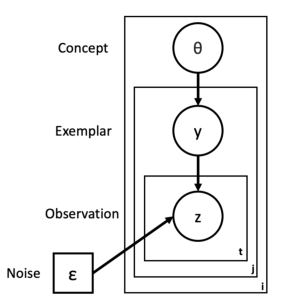
\includegraphics{figs/plate_diagram-1} 

}

\caption[Graphical representation of our model]{Graphical representation of our model. Circles indicate random variables. The squares indicate fixed model parameters.}\label{fig:plate_diagram}
\end{figure}
\end{CodeChunk}

\hypertarget{sampling}{%
\paragraph{Sampling}\label{sampling}}

The formulation of the model in continuous time allows us to do two
things: First, we can explicitly model the learner's decision on when to
stop sampling by asking the model to decide, after every sample \(z\),
whether it wants to continue sampling from the same stimulus or not.
This is in contrast to the discrete time models presented here and in
previous work (Kidd et al., 2012; Poli et al., 2020), where we can only
link information-theoretic measures to looking data, but not provide a
mechanism for how these measures could control moment-to-moment sampling
decisions. Second, a consequence of making a decision at every time step
is that we can study the behavior of another information-theoretic
measure: the expected information gain (EIG). EIG is commonly used in
rational analyses of information-seeking behavior - that is to assess
whether information-seeking is optimal with respect to the learning task
(Markant \& Gureckis, 2012; Oaksford \& Chater, 1994). Importantly, EIG
is a forward-looking measure that considers the potential for learning
from the next sample. Since discrete time models operate on the level of
a whole stimulus, rather than individual samples, EIG would look forward
to the next stimulus in these models, rather than the next sample, and
therefore not be able to capture the decision of whether to keep
looking. EIG to describe looking time is therefore only possible in the
continuous time models.

We compute EIG by weighing the information gain from each possible next
observation by the probability of that observation. We defined
information gain as the KL-divergence between the hypothetical posterior
after observing a sample \(z_{t+1}\) and the current posterior:
\begin{eqnarray}
EIG(z_{t+1}) = \sum_{z_{t+1} \in [0,1]} p(z_{t+1}|\theta_t) * KL(\theta_{t+1}, p(\theta_t))
\end{eqnarray} Finally, to get actual sampling behavior from the model,
it has to convert EIG into a binary decision about whether continue
looking at the current sample, or to advance to the next trial. The
model does so using a luce choice between the EIG from the next sample
and a constant EIG from looking away. \begin{eqnarray}
p(look) = \frac{EIG(z_{t+1})}{EIG(z_{t+1})+EIG(world)}
\end{eqnarray} We also studied the behavior of the model when replacing
EIG with continuous time versions of the other linking hypotheses,
surprisal and KL-divergence between the posterior \(p(\theta_t)\) and
the prior \(p(\theta_{t-1})\).

\hypertarget{experiment}{%
\section{Experiment}\label{experiment}}

\hypertarget{methods}{%
\subsection{Methods}\label{methods}}

\hypertarget{participants}{%
\subsubsection{Participants}\label{participants}}

We recruited 449 participants (Age \emph{M} = 30.83; \emph{SD} = 17.44)
on Prolific. They were randomly assigned to one of the three conditions
of the experiment (Curiosity: \emph{N} = 156; Memory: \emph{N} = 137;
Math: \emph{N} = 156). Participants were excluded if they showed
irregular reaction times or their responses in the filler tasks
indicates low engagement with the experiment. All exclusion criteria
were pre-registered. The final sample included N participants (Curiosity
\emph{N} = 143; Memory: \emph{N} = 98; Math: N = \emph{N} = 139).

\hypertarget{procedure}{%
\subsubsection{Procedure}\label{procedure}}

This is a web-based self-paced visual presentation task. Participants
were instructed to look at a sequence of animated creatures at their own
pace and answer some questions throughout. At the end of the experiment,
participants were asked to rate the similarity between pairs of
creatures and complexity of creatures they encountered on a 7-point
Likert Scale. Each participant saw eight blocks in total, half of which
used creatures with high perceptual complexity, and half of which used
creatures with low perceptual complexity. On each trial, an animated
creature showed up on the screen. participants can press the down arrow
to go to the next trial whenever they want after a minimum viewing time
of 500 ms.

Each block consisted of six trials. A trial can be either a background
trial (B) or a deviant trial (D). A background trial presented a
creature repeatedly, and the deviant trial presented a different
creature from the background trial in the block. Two creatures in the
blocks were matched for visual complexity. There were four sequences of
background trials and deviant trials. Each sequence appeared twice, once
with high complexity stimuli and once with low complexity stimuli. The
deviant trial can appear at either the second (BDBBBB), the fourth
(BBBDBB), or the sixth trial (BBBBBD) in the block. Two blocks do not
have deviant trials (BBBBBB). The creatures presented in the deviant
trials and background trials were matched for complexity. An overview of
the experimental design can be seen in Figure
@ref(fig:experimental\_design).

\begin{CodeChunk}
\begin{figure}[H]

{\centering 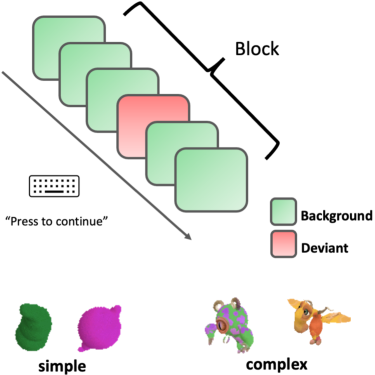
\includegraphics{figs/experimental_design-1} 

}

\caption[Experimental design and examples of simple and complex stimuli]{Experimental design and examples of simple and complex stimuli. In each block, a deviant could appear on the second, fourth (as depicted here) or sixth trial or not at all. Stimuli within a block were either all simple or all complex.}\label{fig:experimental_design}
\end{figure}
\begin{CodeOutput}
{#fig:experimental_design}
\end{CodeOutput}
\end{CodeChunk}

Participants were randomly assigned to one of the three conditions:
Curiosity, Memory, and Math The three conditions only differed in the
type of questions asked following each block. In Curiosity condition,
participants were asked to rate ``How curious are you about the
creature?'' on a 5-point Likert scale. In Memory condition, a
forced-choice recognition question followed each block (``Have you seen
this creature before?''). The creature used in the question in both
conditions was either a creature presented in the preceding block or a
novel creature matched in complexity. In Math condition, the
participants were asked a simple arithmetic question (``What is 5 +
7?'') in multiple-choice format.

\hypertarget{stimuli}{%
\subsubsection{Stimuli}\label{stimuli}}

\begin{CodeChunk}
\begin{figure}[H]

{\centering 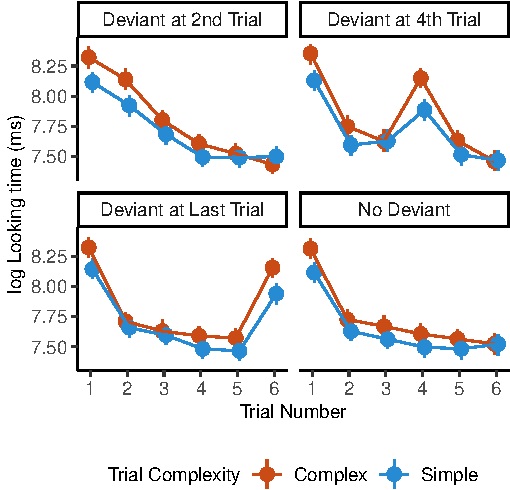
\includegraphics{figs/behavioral_result-1} 

}

\caption[Results of behavioral experiment]{Results of behavioral experiment.}\label{fig:behavioral_result}
\end{figure}
\end{CodeChunk}

The animated creatures (Fig 1) were created using Spore (a game
developed by Maxis in 2008). There were forty creatures in total, half
of which have low perceptual complexity (e.g.~the creatures do not have
limbs, additional body parts, facial features, or textured skin), and
half of which have high perceptual complexity (i.e.~they do have the
aforementioned features). We used the ``animated avatar'' function in
Spore to capture the creatures in motion.

\hypertarget{results}{%
\subsection{Results}\label{results}}

\hypertarget{analytic-approach}{%
\subsubsection{Analytic Approach}\label{analytic-approach}}

The sample size, methods, and main analyses were all pre-registered and
are available at {[}LINK{]}. Data and analysis scripts are available at
{[}LINK{]}.

\hypertarget{manipulation-check}{%
\subsubsection{Manipulation Check}\label{manipulation-check}}

The complex animated creatures were rated as more perceptually complex
(M = ; SD = ) than the simple animated creatures (M = ; SD = ). Pairs of
background creature and deviant creature were rated as moderately
dissimilar to one another (M = ; SD = ).

\hypertarget{evaluating-the-paradigm}{%
\subsubsection{Evaluating the Paradigm}\label{evaluating-the-paradigm}}

Three criteria were selected to evaluate whether the paradigms
successfully captured the characteristic looking time patterns observed
in infant literature: habituation (the decrease in looking time for a
stimulus with repeated presentations), dishabituation (the increase in
looking time to a new stimulus after habituated to one stimulus), and
complexity effect (longer looking time for perceptually more complex
stimuli). To evaluate the phenomenon quantitatively, we ran a linear
mixed effects model with maximal random effect structure. {[}DESCRIBE
THE MODEL{]}. {[}REPORT THE MODEL RESULTS{]}

\hypertarget{discussion}{%
\subsection{Discussion}\label{discussion}}

\hypertarget{model-comparison}{%
\section{Model comparison}\label{model-comparison}}

\hypertarget{parameter-estimation}{%
\subsection{Parameter estimation}\label{parameter-estimation}}

We performed an iterative grid search in parameter space for each
linking hypothesis. We a priori constrained our parameter space on the
prior beta distribution to have shape parameters that
\(\alpha_{\theta} > \beta_{\theta}\), which describe the prior beliefs
as ``more likely to see the absence of a feature than the presence of a
feature.'' For model 1, we searched for the priors over the concept to
be learned. The parameter search for the two metrics, surprisal and
KL-divergence, converged on the same priors (\(\alpha_{\theta}\) =
1;\(\beta_{\theta}\) = 2). For model 2, we searched for the priors over
the concept (\(\theta\)), the noise parameter that decides how likely a
feature would be misperceived (\(\epsilon\)), and the constant EIG from
the world (\(EIG(world)\)). The prior over the noise parameter was fixed
for all searches (\(\alpha_{\epsilon}\) = 1;\(\beta_{\epsilon}\) = 10).
In model 2, different parameters were selected to obtain the best fit to
the behavioral data (EIG: \(\alpha_{\theta}\) = 1, \(\beta_{\theta}\) =
4, \(\epsilon\) = 0.065, \(EIG(world)\) = 0.01; KL: \(\alpha_{\theta}\)
= 1, \(\beta_{\theta}\) = 5, \(\epsilon\) = 0.055, \(EIG(world)\) =
0.006; Surprisal: \(\alpha_{\theta}\) = 1, \(\beta_{\theta}\) = 3,
\(\epsilon\) = 0.07, \(EIG(world)\) = 8).

\begin{CodeChunk}
\begin{figure}[H]

{\centering 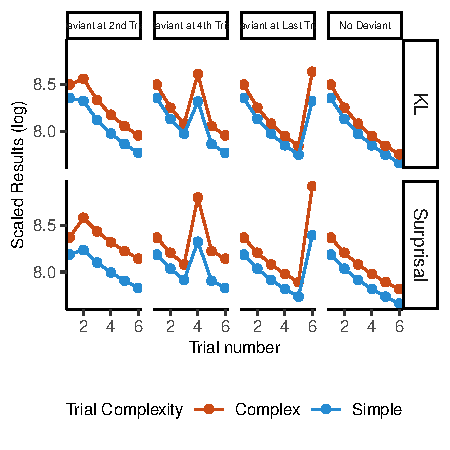
\includegraphics{figs/basic_result-1} 

}

\caption[Results from the discrete time model]{Results from the discrete time model. The top panels show the trajectories of KL under different sequences, and the bottom panels showw the trajectoreis of surprisal.}\label{fig:basic_result}
\end{figure}
\end{CodeChunk}

\hypertarget{model-experiment}{%
\subsection{Model experiment}\label{model-experiment}}

To model the behavioral experiment, we first represented the stimuli as
a vector of logical values indicating the presence and absence of a
feature. All stimuli vectors are length 6, with the complex stimuli
represented as having three \texttt{TRUE} and simple stimuli represented
as having one \texttt{TRUE}, The rest of the elements are
\texttt{FALSE}. Individual stimuli are then assembled into sequences to
reflect the stimuli sequences in the behavioral experiment. For a
particular sequence, we constructed the deviant stimulus based on the
background stimulus to make sure that they were always maximally
different and had the same number of features present.

For Model 1, since it's behavior is non-probabilistic, we presented the
model with each of the four sequences once and derived the information
theoretic measurements. For model 2, we ran each sequence 500 times to
obtain a reasonably precise estimate on the model's behaviors.

\begin{CodeChunk}
\begin{figure*}[h!]

{\centering 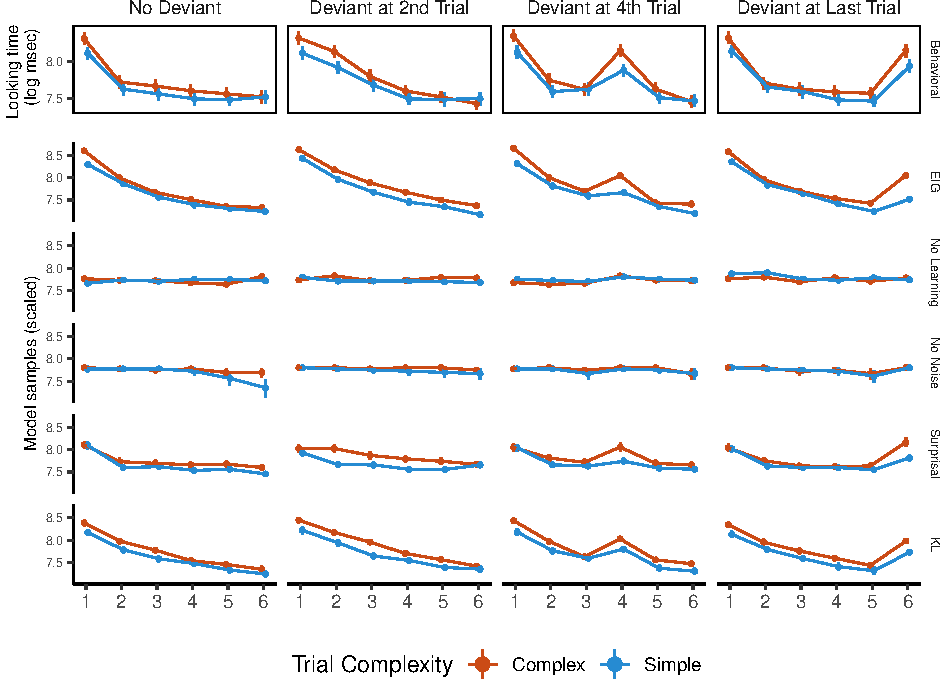
\includegraphics{figs/experiment_res-1} 

}

\caption[Continuous time model using different linking hypotheses provide qualitatively indistinguishable fits to the behavioral data]{Continuous time model using different linking hypotheses provide qualitatively indistinguishable fits to the behavioral data. All model results are log-transformed and adjusted to be at the same scale and intercepts as the log-transformed behavioral data. The solid lines represent human data, and the dotted lines represent the model's results. Red lines indicated results for complex stimuli, and blue lines indicated results for simple stimuli.}\label{fig:experiment_res}
\end{figure*}
\end{CodeChunk}

\hypertarget{results-and-discussion}{%
\subsection{Results and Discussion}\label{results-and-discussion}}

Both models reproduced the behavioral phenomena qualitatively, showing
habituation, dishabituation, and complexity effect. To quantitatively
explore the models, we fit the models' output to the behavioral data.
All models' results were adjusted to match behavioral data's scale and
intercepts for easier comparisons. In model 1, we found that KL provided
a better fit for the behavioral data than surprisal (Fig X; KL: \emph{r}
= 0.9; RMSE = 0.39; Surprisal: \emph{r} = 0.74; RMSE = 0.42) In model 2,
however, we found that the three linking hypotheses were qualitatively
indistinguishable in their fits (Fig X; EIG: \emph{r} = 0.92, RMSE =
0.19; KL: \emph{r} = 0.93, RMSE = 0.12; Surprisal: \emph{r} = 0.92, RMSE
= 0.13). In this section, we discuss the implications of our findings
and future directions.

First, the result from our discrete model extended the Poli et al
(2020)'s findings. We showed in a new behavioral dataset that, similar
to infants, adults' attention allocation is better predicted by KL
divergence than surprisal. This converging finding suggests a
developmental continuity on principles guiding information-seeking
behaviors. Second, the result from our continuous time model is the
first evidence showing that under certain model architecture, surprisal
and KL-divergence are good proxies for EIG, a metric that has the
distinct advantage of quantitatively characterizing the optimal
exploratory behaviors in humans. Tracking EIG can be computationally
expensive and psychologically implausible. To calculate EIG, the current
model needs to consider all possible combinations of features for the
next observation. The proximities of model fits between EIG, KL, and
surprisal revealed an opportunity to further optimize learning policies
for computational models. Further, it also calls for more investigations
on the relationships between different information theoretic metrics'
roles in predicting human behaviors. Our finding is in sharp contrast
with previous work that tries to dissociate between different metrics
using the same behavioral dataset (Poli, Emily). It would be
theoretically interesting to consider under what circumstances do the
measurements converge or become dissociable. Last but not least,
although we can not directly compare the two models' fits quantitatively
due to the differences in the number of free parameters, our results
still show how models' architectural differences can lead to different
conclusions about the linking hypotheses. In a more psychologically
realistic modeling regime, different information theoretic measurements
can become indistinguishable.

There are several limitations to the current work. For our behavioral
data, one concern is that our self-paced visual presentation task might
not be capturing participants' intrinsic interests in exploring the
stimuli, which raises the question on whether we are actually measuring
looking time. We addressed this question by including different filler
tasks in-between blocks. No differences in looking time patterns are
found across conditions. This suggests that the recorded-behaviors are
task demand-independent, which means that they are more likely to
reflect participants' genuine interests in looking at the stimuli. For
our models, there are several limitations that require further
investigation. The current stimuli representation is rather
oversimplified. For example, we did not take into consideration how
features can have different degrees of saliency. In addition, the
sampling policy's implementation can be further challenged. The model
currently decides between ``continuing looking'' and ``look away,'' but
one can argue that in the behavioral experiment the participants were
deciding between ``continuing looking at the current stimulus'' and
``look at the next stimulus.'' Building these more sophisticated
assumptions into the model would certainly help us understand looking
time better under a rational analysis framework. Nevertheless, our
current work suggests that simpler models are capable of explaining key
phenomena in looking time change.

Our ultimate goal is to provide a computational model that can explain
the key looking time patterns documented and utilized in infant
research: habituation, dishabituation, and complexity effect. We believe
these patterns are driven by information-seeking principles that have
strong developmental continuities. In the current work, we have shown
that information theoretic measurements can be linked to adult looking
time patterns. We also compared the two models and found that model
architecture has consequences for linking hypotheses. Specifically, in a
discrete time model, we found KL is a better predictor than surprisal.
But in the continuous time model, three measurements (EIG, KL, and
surprisal) become indistinguishable. As we further elaborate on our
modeling approach, our ongoing work on infants will eventually help
address the developmental trajectories of the mechanisms through which
learners decide what to look at , and when to stop looking.

\hypertarget{references}{%
\section{References}\label{references}}

\hypertarget{references-1}{%
\section{References}\label{references-1}}

\setlength{\parindent}{-0.1in} 
\setlength{\leftskip}{0.125in}

\noindent

\hypertarget{refs}{}
\begin{CSLReferences}{1}{0}
\leavevmode\vadjust pre{\hypertarget{ref-goodman2008rational}{}}%
Goodman, N. D., Tenenbaum, J. B., Feldman, J., \& Griffiths, T. L.
(2008). A rational analysis of rule-based concept learning.
\emph{Cognitive Science}, \emph{32}(1), 108--154.

\leavevmode\vadjust pre{\hypertarget{ref-kidd2012goldilocks}{}}%
Kidd, C., Piantadosi, S. T., \& Aslin, R. N. (2012). The goldilocks
effect: Human infants allocate attention to visual sequences that are
neither too simple nor too complex. \emph{PloS One}, \emph{7}(5),
e36399.

\leavevmode\vadjust pre{\hypertarget{ref-markant2012does}{}}%
Markant, D., \& Gureckis, T. (2012). Does the utility of information
influence sampling behavior? In \emph{Proceedings of the annual meeting
of the cognitive science society} (Vol. 34).

\leavevmode\vadjust pre{\hypertarget{ref-oaksford1994rational}{}}%
Oaksford, M., \& Chater, N. (1994). A rational analysis of the selection
task as optimal data selection. \emph{Psychological Review},
\emph{101}(4), 608.

\leavevmode\vadjust pre{\hypertarget{ref-poli2020infants}{}}%
Poli, F., Serino, G., Mars, R., \& Hunnius, S. (2020). Infants tailor
their attention to maximize learning. \emph{Science Advances},
\emph{6}(39), eabb5053.

\leavevmode\vadjust pre{\hypertarget{ref-tenenbaum1999bayesian}{}}%
Tenenbaum, J. B. (1999). Bayesian modeling of human concept learning.
\emph{Advances in Neural Information Processing Systems}, 59--68.

\end{CSLReferences}

\bibliographystyle{apacite}


\end{document}
